\section{Resultados}

% 10 kbits/s

No presente capítulo, são apresentados os resultados obtidos, a partir da observação do funcionamento do protótipo construído. Serão apresentados imagens demonstrando o funcionamento e além disso serão destacados os desafios enfrentados durante o processo e as estratégias adotadas para mitigá-los.

\subsection{Resultados}

Ao implementar o protocolo \textit{start-stop} o primeiro resultado obtido foram caracteres recebidos diferentes do enviado. A causa do erro foi o tempo de leitura do receptor que ao ler o codigo de start, que é representado pelo byte 11111110, o ultimo bit estava sendo considerado como parte da mensagem.

\begin{figure}[!htbp]
  \caption{As informações mostradas pelo emissor e receptor não correspondem}
  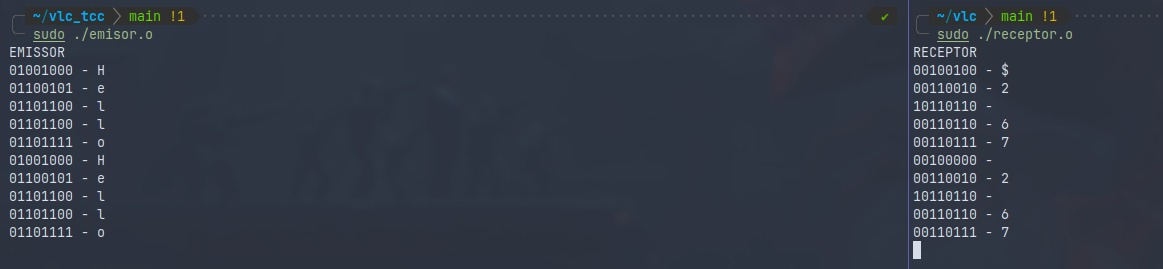
\includegraphics[width=0.9\textwidth]{images/vlc_erro_1.jpeg}
  \legend{Fonte: Autor (2023)}
  \label{primeiro_erro}
\end{figure}

\begin{figure}[!htbp]
  \caption{Comparação entre os bytes enviados e recebidos}
  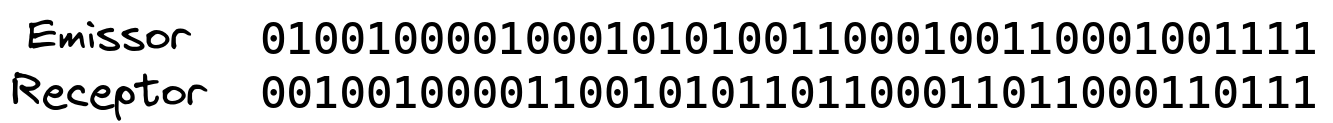
\includegraphics[width=0.9\textwidth]{images/comparacao_msg_emissor_recptor_erro.png}
  \legend{Fonte: Autor (2023)}
  \label{comparaca_msg_emissor_recptor_erro}
\end{figure}

Corrigindo o erro de temporização a transmissão ocorre sem falhas, os 5 bytes são enviados corretamente. A taxa de transmissão foi de 10 bits/s. Não foi possivel atingir taxas maiores pois a SBCs não consegue atingir leituras mais rapidas e o circuito também tem um tempo de resposta não muito favoravel.

\begin{figure}[!htbp]
  \caption{Transmissão correta da mensagem}
  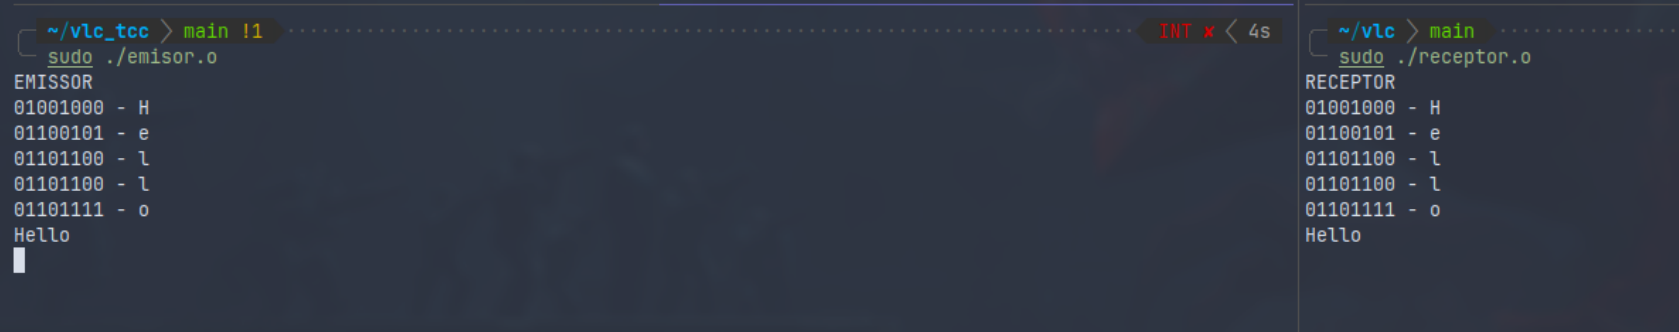
\includegraphics[width=0.8\textwidth]{images/vlc_run.png}
  \legend{Fonte: Autor (2023)}
  \label{vlc_funcionando}
\end{figure}

\newpage

\subsection{Desafios}
